\chapter{Statistics of the South Flood-North Drought: A new catalog of rainbands in the East Asian monsoon}

%consider uploading your actual code to this chapter for reproducibility.

\section{Abstract}
Changes in rainfall can be traced to changes either in the frequency of events, or in their mean intensity. However, according to \cite{Biasutti2011}, the instantaneous strength of rainfall does not change with time - therefore, long-term changes can be traced to changes in frequency.

\section{Climatology of the Meiyu Front}

\section{A Novel Image Processing Algorithm}

\section{Statistics of China Frontal events}

\begin{figure}[htb]

\noindent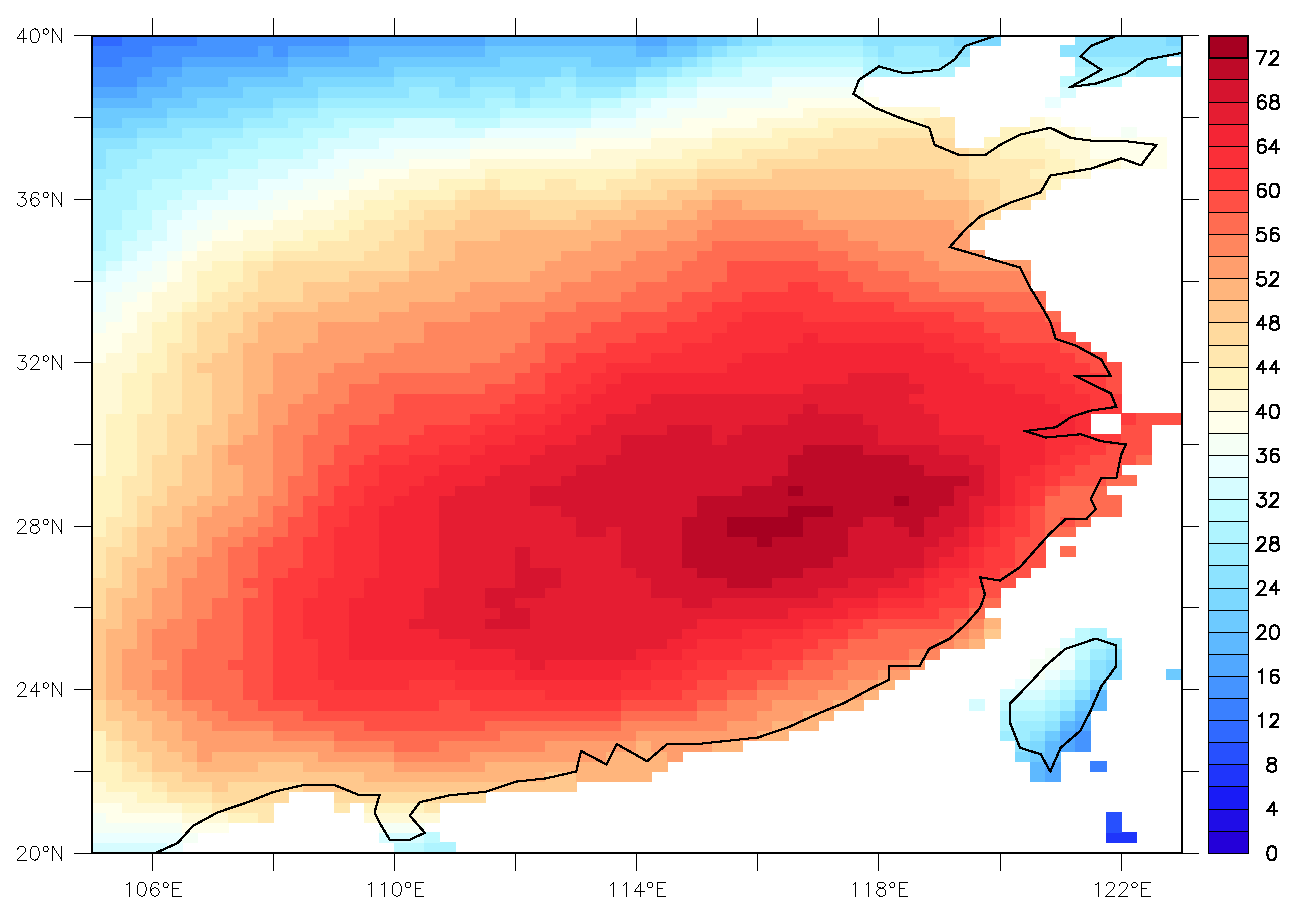
\includegraphics[width=36pc]{Figures/A1_frontpct}
\caption{1980-2007 versus 1951-1979 changes in frontal and local rainfall for full year (a and b), Pre-Meiyu (c and d) and Post-Meiyu (e and f)}
\end{figure}


\section{Calculating the statistical significance of changes: Bootstrapping methods}
The distribution of rainband latitude and intensity during a given season is not constrained to follow a normal distribution. Therefore, in the estimation of statistical significance we are required to employ non-parametric tests. In this chapter, estimations of significance were obtained using bootstrapping with and without replacement (the latter also known as a permutation method), well-established techniques that allow the estimation of relevant quantities by constructing synthetic distributions.

Furthermore, rainband statistics are not independent from one day to the next, but rather exhibit temporal autocorrelation greater than 1. Intuitively from our knowledge of weather, the observation of a front at a particular latitude makes it more likely that it will be subsequently observed at the same latitude. We employ a technique known as a moving blocks bootstrap, described for instance in citep{Singh}. In this case, data are drawn in sequential blocks of $n$ days depending on the strength of the temporal autocorrelation. The choice of block length $n$ is a subject of substantial debate in the statistical literature, but in practice, the choice of block length ranging from 2 to 5 days does not substantially alter our estimations of statistical significance, although in general the choice of longer blocks tends to return the estimated p-value closer to .5.

In our case, we face the added problem that not all variables are continuous in time. If no front is observed on a day then we cannot report a latitude or intensity. In this case we have relied on a regular permutation test, because there is no existing convention to our knowledge for handling the case of missing observations in a moving blocks bootstrap.

Below we attach the relevant code used to perform bootstrapping with replacement, without replacement (permutation test) and the moving blocks bootstrap.

\section{Signature of the ``South Flood-North Drought''}
\subsection{1951-1979 v 1980-2007}
\subsection{1979-1993 v 1994-2007}

\section{Comparison with alternative metrics}
It is reasonable to suggest that some simpler metric ought to exist that reproduces the results of the Rainband Detection Algorithm (RDA). In this section, we test a suite of simple metrics, using the same bootstrapping algorithms used to calculate the statistical significance of changes in observed yearly rainfall. These metrics are as follows: ...

The following figure demonstrates the climatology of the 8 metrics described above:

\begin{figure}[htb]

\noindent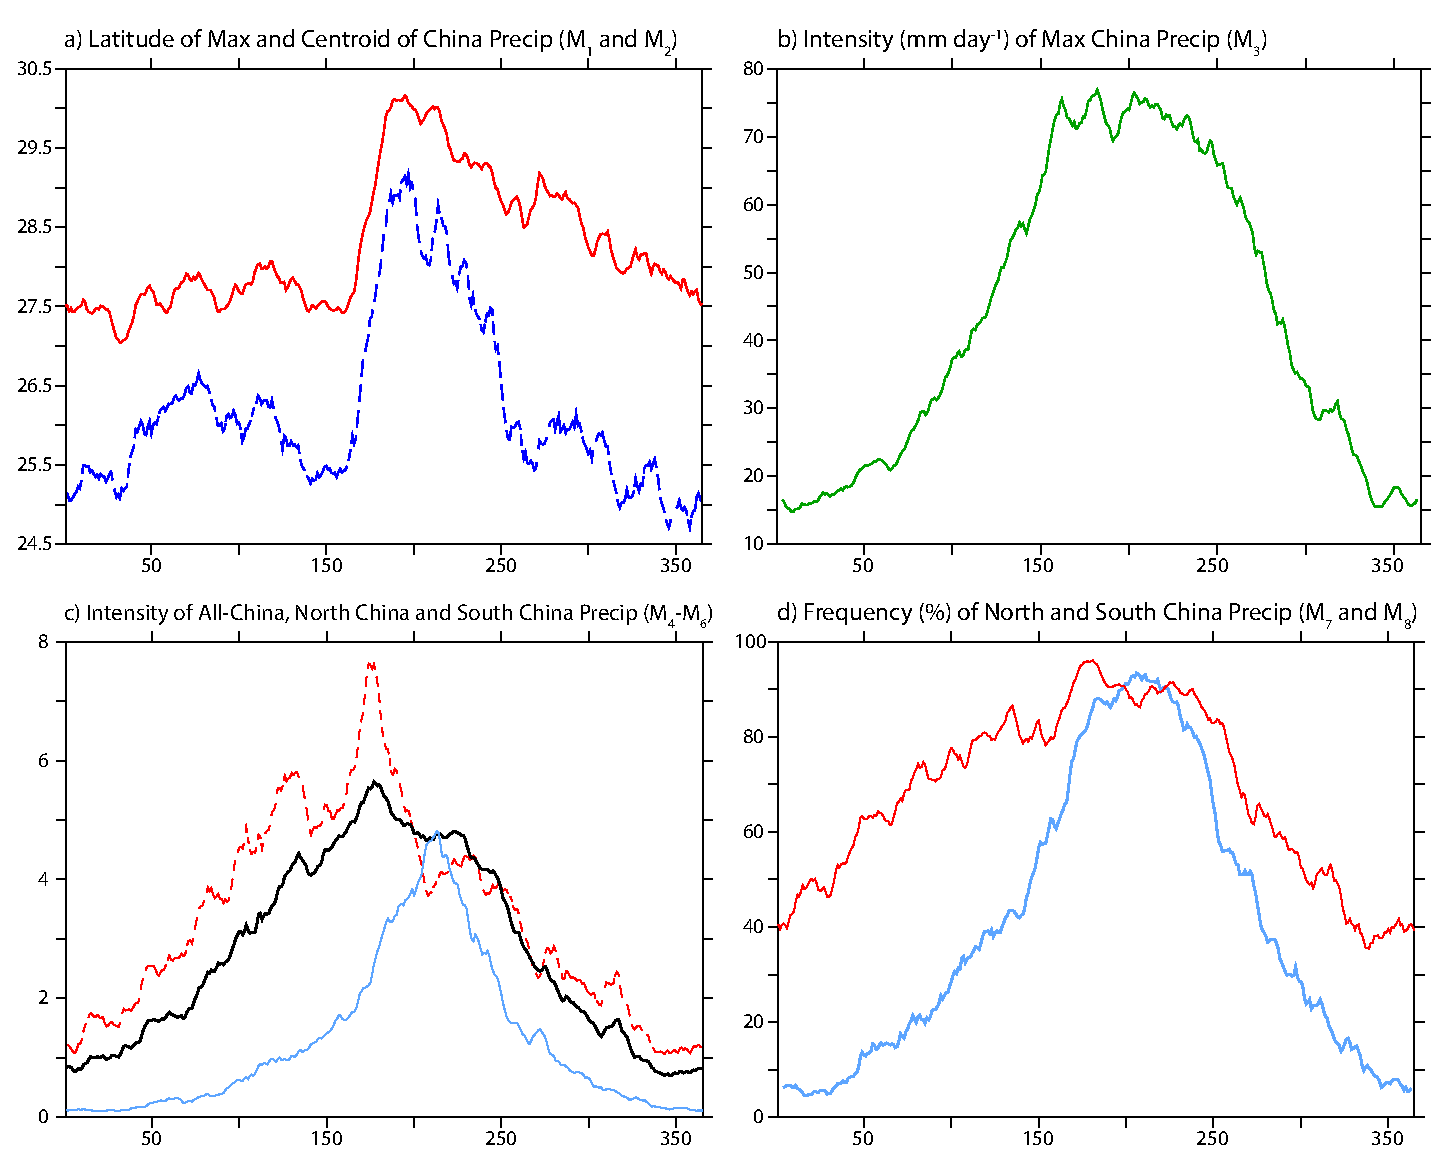
\includegraphics[width=36pc]{Figures/A3_met_climo}
\caption{1980-2007 versus 1951-1979 changes in frontal and local rainfall for full year (a and b), Pre-Meiyu (c and d) and Post-Meiyu (e and f)}
\end{figure}



%%%% ALTERNATIVE METRIC STATISTICS, 1951-1979 %%%%
\begin{table}[p]

\centering

\caption{Mean and standard deviation of mean of metrics $M_1$ to $M_8$ for 1951-1979 as previously defined. Standard deviations of means are obtained by a permutation method with 10,000 iterations. Statistically significant changes at the 95\%/99\% level are indicated by bold/asterisk and bold as subsequently calculated in Table S12.}

\begin{tabular}{ l c c c c c c c c}
	 \multicolumn{9}{c}{\textbf{1951-1979 Means}}  \\
	 \textbf{Time Period} 						& $\boldsymbol{M_1}$ & $\boldsymbol{M_2}$ & $\boldsymbol{M_3}$ & $\boldsymbol{M_4}$ & $\boldsymbol{M_5}$ & $\boldsymbol{M_6}$ & $\boldsymbol{M_7}$ & $\boldsymbol{M_8}$ \\
	 \hline
	\textbf{Spring Rains} (Mar 1-Apr 30, 60-120) 	& $26.3 \pm 0.2$ 	&  $\boldsymbol{27.9 \pm 0.1}$	&  $31.2 \pm 1.1$ 	&$2.6 \pm 0.1$ 	& $.52 \pm 0.05$ 		& $3.9 \pm .2$ & $25.0 \pm 2.0$ & $71.7 \pm 2.1$  \\
	\textbf{Pre-Meiyu} (May 1-Jun 9, 121-160) 		& $25.7 \pm 0.2$ 	&  $27.6 \pm 0.1$				&  $59.4 \pm 1.9$ 	&$4.4 \pm 0.2$	& $1.20 \pm 0.11$ 	& $5.5 \pm .3$ & $47.1 \pm 3.0$ & $82.6 \pm 2.2$ \\
	\textbf{Meiyu} (Jun 10-Jul 19, 161-120) 		& $27.9 \pm 0.3$ 	&  $29.1 \pm 0.2$				&  $72.5 \pm 2.1$ 	&$5.1 \pm 0.1$ 	& $2.78 \pm 0.18$		& $5.9 \pm .3$ & $81.1 \pm 2.4$ & $91.0 \pm 1.7$ \\
	\textbf{Post-Meiyu} (Jul 20-Sep 30) 			& $27.4 \pm 0.3 $	&  $29.4 \pm 0.1$ 				&  $69.1 \pm 1.9$ 	&$4.1 \pm 0.1$ 	& $\boldsymbol{3.20 \pm 0.16^*}$		& $3.7 \pm .2$ & $76.4 \pm 1.8$ & $82.0 \pm 1.7$ \\
	\textbf{Fall Rains} (Oct 1-Nov 16) 				& $25.6 \pm 0.2 $ 	&  $28.5 \pm 0.2$				&  $36.9 \pm 1.8$ 	&$1.9 \pm 0.1$	& $.76 \pm 0.09$ 		& $2.3 \pm .2$ & $30.7 \pm 2.5$ & $57.2 \pm 2.6$ \\
	\textbf{Full Year} (1-365) 					& $26.2 \pm 0.1$ 	&  $28.3 \pm 0.1$ 				&  $43.5 \pm 0.7$ 	&$2.8 \pm 0.1$ 	& $\boldsymbol{1.31 \pm 0.05}$		& $3.4 \pm .1$ & $40.0 \pm 1.0$ & $67.7 \pm 1.0$ \\
\end{tabular}
\label{ts4}
\end{table}


%%%% TABLE 10 - ALTERNATIVE METRIC STATISTICS, 1980-2007 %%%%
\begin{table}[p]

\centering

\caption{Mean and standard deviation of mean of metrics $M_1$ to $M_8$ for 1980-2007 as previously defined. Standard deviations of means are obtained by a permutation method with 10,000 iterations. Statistically significant changes at the 95\%/99\% level are indicated by bold/asterisk and bold as subsequently calculated in Table S12.}

\begin{tabular}{ l c c c c c c c c}
	 \multicolumn{9}{c}{\textbf{1980-2007 Means}} \\
	 \textbf{Time Period} 						& $\boldsymbol{M_1}$ & $\boldsymbol{M_2}$ 		& $\boldsymbol{M_3}$ & $\boldsymbol{M_4}$ & $\boldsymbol{M_5}$ & $\boldsymbol{M_6}$ & $\boldsymbol{M_7}$ & $\boldsymbol{M_8}$ \\	 \hline
	\textbf{Spring Rains} (Mar 1-Apr 30, 60-120)  	& $26.2 \pm 0.2$ 	&  $\boldsymbol{27.6 \pm 0.1}$	&  $32.4 \pm 1.0$ 	&$2.6 \pm 0.1$ 	& $.51 \pm 0.06$ 		& $3.8 \pm .2$ & $24.1 \pm 2.1$ & $72.5 \pm 2.2$  \\
	\textbf{Pre-Meiyu} (May 1-Jun 9, 121-160)  	& $25.4 \pm 0.2$ 	&  $27.7 \pm 0.2$				&  $57.0 \pm 1.8$ 	&$4.2 \pm 0.2$	& $1.31 \pm 0.12$ 	& $5.0 \pm .3$ & $48.8 \pm 3.0$ & $79.6 \pm 2.4$ \\
	\textbf{Meiyu} (Jun 10-Jul 19, 161-120)		& $27.6 \pm 0.3$ 	&  $29.1 \pm 0.1$				&  $73.6 \pm 2.2$ 	&$5.2 \pm 0.1$ 	& $2.79 \pm 0.18$		& $6.4 \pm .3$ & $81.3 \pm 2.3$ & $92.1 \pm 1.6$ \\
	\textbf{Post-Meiyu} (Jul 20-Sep 30) 			& $27.0 \pm 0.2 $	&  $29.2 \pm 0.1$ 				&  $67.5 \pm 1.9$ 	&$4.0 \pm 0.1$ 	& $\boldsymbol{2.70 \pm 0.14^*}$		& $3.9 \pm .2$ & $75.3 \pm 1.9$ & $85.5 \pm 1.6$ \\
	\textbf{Fall Rains} (Oct 1-Nov 16) 				& $26.0 \pm 0.3 $ 	&  $28.5 \pm 0.2$				&  $36.4 \pm 2.1$ 	&$1.8 \pm 0.1$	& $.65 \pm 0.08$ 		& $2.4 \pm .2$ & $28.0 \pm 2.5$ & $54.7 \pm 2.8$ \\
	\textbf{Full Year} (1-365)					& $26.2 \pm 0.1$ 	&  $28.2 \pm 0.1$ 				&  $43.1 \pm 0.7$ 	&$2.8 \pm 0.1$ 	& $\boldsymbol{1.20 \pm 0.04}$		& $3.4 \pm .1$ & $39.4 \pm 1.0$ & $68.6 \pm 1.0$ \\
\end{tabular}
\label{ts4}
\end{table}


%%%% TABLE 11 - AUTOCORRELATION TIME SCALE OF ALTERNATIVE METRICS %%%%
\begin{table}[p]

\centering

\caption{Autocorrelation timescale of metrics $M_1$-$M_8$, calculated as described in section S2. In subsequent calculations of significance, the block length for moving blocks bootstrapping is chosen}

\begin{tabular}{ l c c c c c c c c}
	 \multicolumn{9}{c}{\textbf{1980-2007 Means}} \\
	 \textbf{Time Period} 						& $\boldsymbol{M_1}$ & $\boldsymbol{M_2}$ & $\boldsymbol{M_3}$ & $\boldsymbol{M_4}$ & $\boldsymbol{M_5}$ & $\boldsymbol{M_6}$ & $\boldsymbol{M_7}$ & $\boldsymbol{M_8}$ \\	 \hline
	 \hline
	\textbf{Spring Rains} (Mar 1-Apr 30, 60-120) 	& 2.20 & 2.52 & 2.49 & 1.77 & 1.94 & 1.57 & 1.60 & 1.92 \\
	\textbf{Pre-Meiyu} (May 1-Jun 9, 121-160) 		& 2.08 & 2.22 & 2.02 & 1.97 & 1.66 & 1.66 & 1.92 & 1.92 \\		
	\textbf{Meiyu} (Jun 10-Jul 19, 161-120) 		& 2.71 & 3.65 & 2.32 & 3.38 & 2.22 & 3.47 & 2.01 & 2.10 \\
	\textbf{Post-Meiyu} (Jul 20-Sep 30) 			& 1.93 & 2.76 & 2.05 & 3.20 & 2.31 & 3.24 & 2.13 & 2.46 \\
	\textbf{Fall Rains} (Oct 1-Nov 16) 				& 1.58 & 2.69 & 3.32 & 3.14 & 1.37 & 1.37 & 1.44 & 3.57 \\
	\textbf{Full Year} (1-365)	 				& 2.16 & 3.03 & 2.56 & 2.75 & 2.14 & 2.14 & 1.84 & 2.82 \\
\end{tabular}
\label{ts11}
\end{table}


%% TABLE 12 - p-value of change in metrics M_1-M_8 between 1951-1979 and 1980-2007
\begin{table}[p]

\centering

\caption{Significance level $p$ of changes in metrics $M_1$-$M_8$ between 1951-1979 and 1980-2007, as calculated by a moving blocks bootstrap for latitude and intensity metrics with 10,000 iterations and block length of $\tau$ rounded up to nearest integer, and analytically calculated using effective degrees of freedom N=$n/\tau$ for frequency metrics $M_7$ and $M_8$. Statistically significant changes at the 95\%/99\% level are indicated by bold/asterisk and bold.}

\begin{tabular}{ l c c c c c c c c}
	 \multicolumn{9}{c}{\textbf{1980-2007 Means}} \\
	 \textbf{Time Period} 						& $\boldsymbol{M_1}$ & $\boldsymbol{M_2}$ & $\boldsymbol{M_3}$ & $\boldsymbol{M_4}$ & $\boldsymbol{M_5}$ & $\boldsymbol{M_6}$ & $\boldsymbol{M_7}$ & $\boldsymbol{M_8}$ \\	 \hline
	 \hline
	\textbf{Spring Rains} (Mar 1-Apr 30, 60-120) 	& .180 & \textbf{.017} 	& .850 & .414 	& .346 			& .320 & .298 & .649 \\
	\textbf{Pre-Meiyu} (May 1-Jun 9, 121-160) 		& .077 & .819 			& .080 & .154 & .871 			& .038 & .729 & .091 \\		
	\textbf{Meiyu} (Jun 10-Jul 19, 161-120) 		& .091 & .468 			& .696 & .808 & .503 			& .943 & .538 & .745 \\
	\textbf{Post-Meiyu} (Jul 20-Sep 30) 			& .046 & .150 			& .162 & .132 & \textbf{.0004*} 	& .848 & .296 & .975 \\
	\textbf{Fall Rains} (Oct 1-Nov 16) 				& .965 & .412 			& .442 & .154 & .049 			& .620 & .107 & .244 \\
	\textbf{Full Year} (1-365)	 				& .726 & .068 			& .314 & .302 & \textbf{.0068} 	& .776 & .242 & .784 \\
	
\end{tabular}
\label{ts12}
\end{table}

In summary, alternative metrics do not consistently show twentieth-century changes in China equivalent to those found with the RDA algorithm. Major changes such as the Post-Meiyu decline in North China rainfall are also reflected in a simple area average, but such a technique misses the southward shift in observed rainbands seen in Figure \ref{}. 

\section{Decadal changes in types of rainfall}
The RDA allows the classification of all rainfall on each day into two categories: Frontal/belonging to a rainband, and non-frontal/local. We have therefore created a 57-year data set of rainfall divided into each of the two categories, downloadable from the author's website with the title APHRO_ZH_front_025deg_V1101.year.nc, where ZH denotes China.

The 57-year climatology of each type of rainfall (banded and non-banded) has been compiled into videos that are appended to this thesis, and also available on the author's website at LINK. A comparison of a pure climatology of China rainfall and its equivalent using only rainfall belonging to bands more coherently shows the seasonal transition between Pre-Meiyu and Meiyu rainfall and the northward progression of mean rainfall during June.

In addition, we can also test the statistical significance of the changes in both banded and local rainfall. In the figure below, we show such changes between 1951-1979 and 1980-2007 and calculate statistical significance for full year and the Pre-Meiyu and Post-Meiyu seasons, which contained the largest changes in rainfall. Unsurprisingly, changes in rainband rainfall occur along long continuous bands, while local rainfall changes are considerably patchier in spatial coverage. During the Pre-Meiyu season, we observed a marked decrease in frontal rainfall along the Yangtze River Valley, but also a simultaneous increase in local rainfall in the vicinity of Sichuan Province collocated with the western half of the rainband decrease. This opens the possibility that the skill of our algorithm in classifying rainfall is not consistent between decades. However, in North China both frontal and local rainfall have decreased during the Post-Meiyu. Taiwan has experienced a substantial decline in local rainfall of several mm day$^{-1}$ that cannot be attributed to changes in rainband behavior.

\textcolor{red}{In summary, the North Flood-South Drought is describable primarily via changes in banded rainfall. In turn, these changes in banded rainfall are mostly zonally symmetric and coherent across thousands of kilometers, which suggests that they are caused by changes in larger-scale dynamics.}

\begin{figure}[htb]

\noindent\includegraphics[width=36pc]{Figures/A2_decadal_front}
\caption{1980-2007 versus 1951-1979 changes in frontal and local rainfall for full year (a and b), Pre-Meiyu (c and d) and Post-Meiyu (e and f)}
\end{figure}

